% generated by report/gen_tables.py from build/scene_export.json -- do not edit
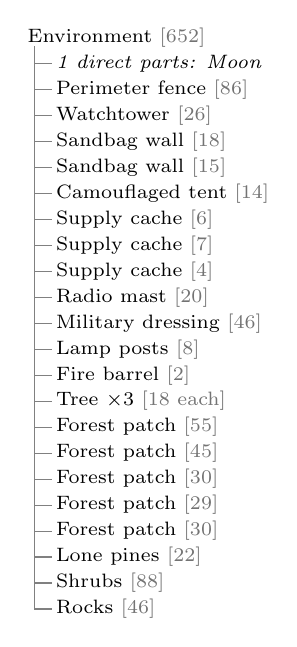
\begin{tikzpicture}[x=0.36cm,y=-0.33cm,font=\scriptsize]
\node[anchor=west,inner sep=0pt] (n0) at (0,0) {Environment \textcolor{black!55}{[652]}};
\node[anchor=west,inner sep=0pt] (n1) at (1,1) {\textit{1 direct parts: Moon}};
\draw[black!50,thin] (0.25,0.35) |- (0.88,1);
\node[anchor=west,inner sep=0pt] (n2) at (1,2) {Perimeter fence \textcolor{black!55}{[86]}};
\draw[black!50,thin] (0.25,0.35) |- (0.88,2);
\node[anchor=west,inner sep=0pt] (n3) at (1,3) {Watchtower \textcolor{black!55}{[26]}};
\draw[black!50,thin] (0.25,0.35) |- (0.88,3);
\node[anchor=west,inner sep=0pt] (n4) at (1,4) {Sandbag wall \textcolor{black!55}{[18]}};
\draw[black!50,thin] (0.25,0.35) |- (0.88,4);
\node[anchor=west,inner sep=0pt] (n5) at (1,5) {Sandbag wall \textcolor{black!55}{[15]}};
\draw[black!50,thin] (0.25,0.35) |- (0.88,5);
\node[anchor=west,inner sep=0pt] (n6) at (1,6) {Camouflaged tent \textcolor{black!55}{[14]}};
\draw[black!50,thin] (0.25,0.35) |- (0.88,6);
\node[anchor=west,inner sep=0pt] (n7) at (1,7) {Supply cache \textcolor{black!55}{[6]}};
\draw[black!50,thin] (0.25,0.35) |- (0.88,7);
\node[anchor=west,inner sep=0pt] (n8) at (1,8) {Supply cache \textcolor{black!55}{[7]}};
\draw[black!50,thin] (0.25,0.35) |- (0.88,8);
\node[anchor=west,inner sep=0pt] (n9) at (1,9) {Supply cache \textcolor{black!55}{[4]}};
\draw[black!50,thin] (0.25,0.35) |- (0.88,9);
\node[anchor=west,inner sep=0pt] (n10) at (1,10) {Radio mast \textcolor{black!55}{[20]}};
\draw[black!50,thin] (0.25,0.35) |- (0.88,10);
\node[anchor=west,inner sep=0pt] (n11) at (1,11) {Military dressing \textcolor{black!55}{[46]}};
\draw[black!50,thin] (0.25,0.35) |- (0.88,11);
\node[anchor=west,inner sep=0pt] (n12) at (1,12) {Lamp posts \textcolor{black!55}{[8]}};
\draw[black!50,thin] (0.25,0.35) |- (0.88,12);
\node[anchor=west,inner sep=0pt] (n13) at (1,13) {Fire barrel \textcolor{black!55}{[2]}};
\draw[black!50,thin] (0.25,0.35) |- (0.88,13);
\node[anchor=west,inner sep=0pt] (n14) at (1,14) {Tree $\times$3 \textcolor{black!55}{[18 each]}};
\draw[black!50,thin] (0.25,0.35) |- (0.88,14);
\node[anchor=west,inner sep=0pt] (n15) at (1,15) {Forest patch \textcolor{black!55}{[55]}};
\draw[black!50,thin] (0.25,0.35) |- (0.88,15);
\node[anchor=west,inner sep=0pt] (n16) at (1,16) {Forest patch \textcolor{black!55}{[45]}};
\draw[black!50,thin] (0.25,0.35) |- (0.88,16);
\node[anchor=west,inner sep=0pt] (n17) at (1,17) {Forest patch \textcolor{black!55}{[30]}};
\draw[black!50,thin] (0.25,0.35) |- (0.88,17);
\node[anchor=west,inner sep=0pt] (n18) at (1,18) {Forest patch \textcolor{black!55}{[29]}};
\draw[black!50,thin] (0.25,0.35) |- (0.88,18);
\node[anchor=west,inner sep=0pt] (n19) at (1,19) {Forest patch \textcolor{black!55}{[30]}};
\draw[black!50,thin] (0.25,0.35) |- (0.88,19);
\node[anchor=west,inner sep=0pt] (n20) at (1,20) {Lone pines \textcolor{black!55}{[22]}};
\draw[black!50,thin] (0.25,0.35) |- (0.88,20);
\node[anchor=west,inner sep=0pt] (n21) at (1,21) {Shrubs \textcolor{black!55}{[88]}};
\draw[black!50,thin] (0.25,0.35) |- (0.88,21);
\node[anchor=west,inner sep=0pt] (n22) at (1,22) {Rocks \textcolor{black!55}{[46]}};
\draw[black!50,thin] (0.25,0.35) |- (0.88,22);
\end{tikzpicture}
